\documentclass[a4paper,10pt, english]{article}
%\usepackage[margin=0.5in]{geometry}
\usepackage[utf8]{inputenc}
\usepackage{amsmath,graphicx,varioref,verbatim,amsfonts,geometry}
\usepackage[norsk]{babel}
\usepackage[usenames,dvipsnames,svgnames,table]{xcolor}
\usepackage[colorlinks]{hyperref}
\usepackage{relsize}
\usepackage{amsmath}
\usepackage{booktabs}

\newcommand*\diff{\mathop{}\!\mathrm{d}}
\newcommand*\Diff[1]{\mathop{}\!\mathrm{d^#1}}
\usepackage{ulem}
\usepackage{amssymb}
\usepackage{soul}
\usepackage{dsfont}
\usepackage{commath}
\usepackage{wrapfig}

\usepackage[free-standing-units=true]{siunitx}
\DeclareSIUnit\year{yr}

%ROMERSKE TALL med \rom
\makeatletter
\newcommand*{\rom}[1]{\expandafter\@slowromancap\romannumeral #1@}
\makeatother

\usepackage{physics}
\usepackage{caption}
\usepackage{bm}
\usepackage[makeroom]{cancel}

\makeatletter
\newcounter{elimination@steps}
\newcolumntype{R}[1]{>{\raggedleft\arraybackslash$}p{#1}<{$}}
\def\elimination@num@rights{}
\def\elimination@num@variables{}
\def\elimination@col@width{}
\newenvironment{elimination}[4][0]
{
    \setcounter{elimination@steps}{0}
    \def\elimination@num@rights{#1}
    \def\elimination@num@variables{#2}
    \def\elimination@col@width{#3}
    \renewcommand{\arraystretch}{#4}
    \start@align\@ne\st@rredtrue\m@ne
}
{
    \endalign
    \ignorespacesafterend
}
\newcommand{\eliminationstep}[2]
{
    \ifnum\value{elimination@steps}>0\sim\quad\fi
    \left[
        \ifnum\elimination@num@rights>0
            \begin{array}
            {@{}*{\elimination@num@variables}{R{\elimination@col@width}}
            |@{}*{\elimination@num@rights}{R{\elimination@col@width}}}
        \else
            \begin{array}
            {@{}*{\elimination@num@variables}{R{\elimination@col@width}}}
        \fi
            #1
        \end{array}
    \right]
    &
    \begin{array}{l}
        #2
    \end{array}
    \addtocounter{elimination@steps}{1}
}
\makeatother
% Document formatting
\setlength{\parindent}{0mm}
\setlength{\parskip}{1.5mm}

%Color scheme for listings
\usepackage{textcomp}
\definecolor{listinggray}{gray}{0.9}
\definecolor{lbcolor}{rgb}{0.9,0.9,0.9}
\newenvironment{Figure}{\par\medskip\noindent\minipage{\linewidth}}{\endminipage\par\medskip}

%Listings configuration
\usepackage{listings}
%\usemintedstyle{emacs}
\lstset{
	backgroundcolor=\color{lbcolor},
	tabsize=4,
	rulecolor=,
	language=python,
        basicstyle=\scriptsize,
        upquote=true,
        aboveskip={1.5\baselineskip},
        columns=fixed,
	numbers=left,
        showstringspaces=false,
        extendedchars=true,
        breaklines=true,
        prebreak = \raisebox{0ex}[0ex][0ex]{\ensuremath{\hookleftarrow}},
        frame=single,
        showtabs=false,
        showspaces=false,
        showstringspaces=false,
        identifierstyle=\ttfamily,
        keywordstyle=\color[rgb]{0,0,1},
        commentstyle=\color[rgb]{0.133,0.545,0.133},
        stringstyle=\color[rgb]{0.627,0.126,0.941}
        }


\title{Mandatory assignement 3\\
FYS2160 - Thermal physics and statistical mechanics}
\author{\textsc{Ivar Svalheim Haugerud}\\University of Oslo}
\date{October 2018}

\begin{document}

\maketitle

\section*{Problem 1 - Van Der Waals Gas}
\subsection*{1.1}
The Helmholtz free energy for the van der Waals gas is given as
\begin{equation}
    F(T, V, N) = -NkT\left(\ln{\left(\frac{V-NB}{N\Lambda^3}\right)}+1\right)-\frac{aN^2}{V}.
\end{equation}
From this the Helmholtz free energy we can derive the equation of state through
\begin{equation}
    P =-\left(\pdv{F}{V}\right)_{T,N}.
\end{equation}
Let's calculate the derivative of the Helmholtz free energy with respect to volume, to find the equation of state
\begin{align*}
    P &= -\left(\pdv{F}{V}\right)_{T,N} \\
      &= -\pdv{}{V}\left(-NkT\left(\ln{\left(\frac{V-NB}{N\Lambda^3}\right)}+1\right)-\frac{aN^2}{V}\right) \\
      &= NkT\pdv{}{V}\left(\ln{\left(\frac{V-NB}{N\Lambda^3}\right)}\right) + NkT\pdv{}{V}\left(1\right) + \pdv{}{V}\left(\frac{aN^2}{V}\right) \\
      &= NkT\left(\frac{1}{\frac{V-Nb}{N\Lambda^3}}\frac{1}{N\Lambda^3}\right) - \frac{aN^2}{V^2} \\
      &= \frac{NkT}{V-Nb} - \frac{aN^2}{V^2}
\end{align*}
Which we recognize as the van der Waal equation.

\subsection*{1.2}
With the equation of state we can find an expression for the work done on the gas when the change in volume compresses from $V_1$ to $V_2$, where $V_2<V_1$.
\begin{align*}
    W &= -\int_{V_1}^{V_2}P \diff V \\
      &= -\int_{V_1}^{V_2} \frac{NkT}{V-Nb} - \frac{aN^2}{V^2} \diff V \\
      &= -NkT \int_{u(V_1)}^{u(V_2)}\frac{1}{u}\diff U  + aN^2\int_{V_1}^{V_2}\frac{1}{V}\diff V \\
      &= -NkT\Bigg[\ln{V-Nb}\Bigg]_{V_1}^{V_2}-aN^2\Bigg[\frac{1}{V}\Bigg]_{V_1}^{V_2} \\
      &= NkT\ln{\left(\frac{V_1-Nb}{V_2-Nb}\right)}+aN^2\left(\frac{1}{V_1}-\frac{1}{V_2}\right)
\end{align*}
We want to compare this work to the work needed to compress an ideal gas the same amount, which is given by
\begin{equation}
    W_{ideal} = NkT\ln{\left(\frac{V_1}{V_2}\right)}.
\end{equation}
We see that if both $a$ and $b$ are zero, the work done is the same for the van der Waals equation and the ideal gas. In the low density limit, where $N$ is large and $V_1$ and $V_2$ is small, the work needed to do for the van der Waals gas larger. This is due to the denominator within the logarithm going towards zero faster than for the ideal gas, as well as the term which goes as $N^2$ making it even harder. This is due to the van der Waal equation taking into account that we can not compress a gas to an infinitely small volume, and the term $-Nb$ is making sure of it. While the ideal gas does not include particle-particle interactions, and is therefore not effected directly by the gas being more dense. \\
For the low density limit, where $N$ is small and $V$ is large the van der Waals term of $aN^2(1/V_1-1/V_2)$ is negligible. In addition the term $-Nb$ will also be nnegligiblecompared to $V_1$ and $V_2$. This means that the van der Waals equation is approximately equal to the ideal gas case. We will therefore get the same work done for both van der Waals equation and ideal gas.
\subsection*{1.3}
We will now use the equation of state to plot the relationship between pressure and volume for different temperatures
\begin{equation}
    T = \{70, 100, 110, 115, 120, 125\}\text{K}. \label{temps}
\end{equation}
The equation will be dimensionless through the critical values
\begin{align*}
    P_c &= 33.6 \text{ atm} \\
    V_c &= 0.089 \text{ l/mol} \\
    T_c &= 126 \text{ K},
\end{align*}
We use the critical values to find an expression for $a$ and $b$ and $N$ through the following equations
\begin{align*}
    P_c &= \frac{a}{27b^2}  \\
    V_c &= 3Nb \\
    kT_c &= \frac{8a}{27b},
\end{align*}
which can be derived by studying at first and second derivatives of the equation of state, and find for what values the derivative is equal to zero. The equations above can be combined to find
\begin{align*}
    b &= \frac{kT_c}{8P_c} \\
    a &= 27P_c\left(\frac{kT_c}{8P_c}\right)^2 \\
    N &= \frac{8P_cV_c}{3kT_c}
\end{align*}
By using these expressions for $a$, $b$ and $N$, we have all the unknowns for our system, and plugging them into equation van der Waals equation makes the equation dimensionless.
In figure \vref{fig:13} we see the pressure as a function of volume for the temperatures given in \eqref{temps}. Where we have used the critical values of pressure, volume and temperature to scale the equation. The code to creates this figure is shown in listing \vref{program1}.

\begin{figure}[h!]
  \centering
    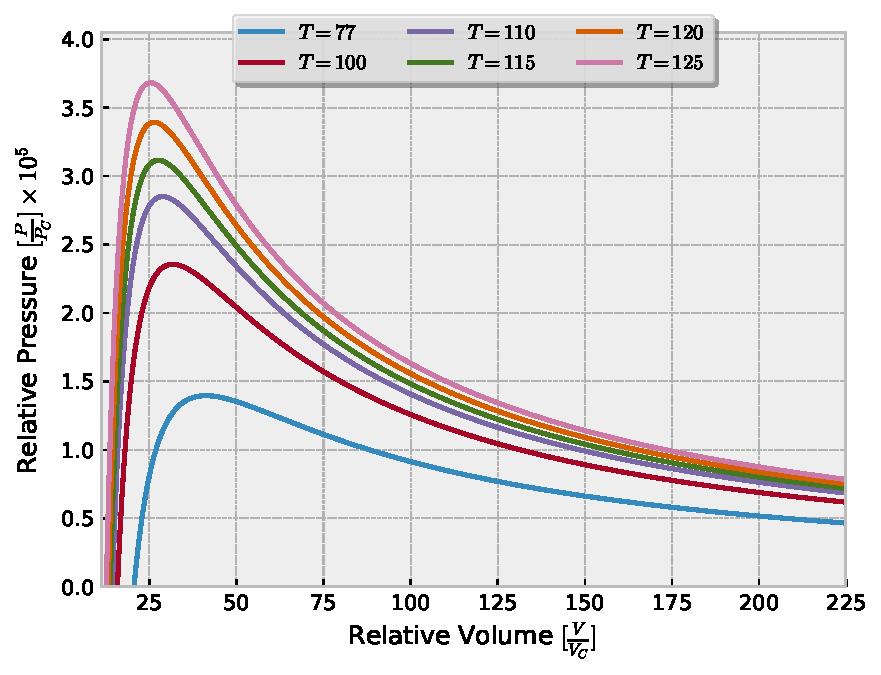
\includegraphics[width=0.8\textwidth]{../figures/equation_of_state.pdf}
    \caption{Relative pressure as a function of relative volume for different temperatures derived analytically from the van der Waals equation. The unit of the temperatures in the legend is kelvin.}
    \label{fig:13}
\end{figure}
In this figure we can see that we observe negative pressure, how is this physically possible? \\For large volumes an increase in volume does not effect the pressure by any measurable amount. This is the behaviour of a gas. For small volumes on the other hand, a small increase in volume results in a huge change in pressure. This is the behaviour of a liquid. This means that for the right side of the graph shown in figure \vref{fig:13} we have a gas, and on the left side we have a liquid. The figure therefore shows us the transition from gas to liquid. The phase transition is the reason for the negative pressure. During the phase transition the change in volume will not change the pressure, but rather help with the phase transition from gas to liquid. The \textit{true} graph would look more like what we observe for the ideal gas, $1/V$. The negative pressure is therefore not what we would observe in an experiment, where the pressure would stay fixed during the phase transition, and after the phase transition we would then observe a large change when we try to compress the volume. We will study this closer in the next problem.
\subsection*{1.4}
We want to use the Maxwell construction for equal area to determine the liquid volume $V_l$ and gas volume $V_g$ for a given temperature. To find the area under the graph we write an algorithm. The algorithm loops over different values of the pressure, and find the corresponding volume values which the pressure intersects the P-V graph. We then use the trapezoidal method to calculate the area under the graph. We calculate the difference in area, and for each temperature we find the pressure value which results in the smallest difference in area. This area is plotted for all temperatures in figure \vref{fig:14}.
\begin{figure}[h!]
  \centering
    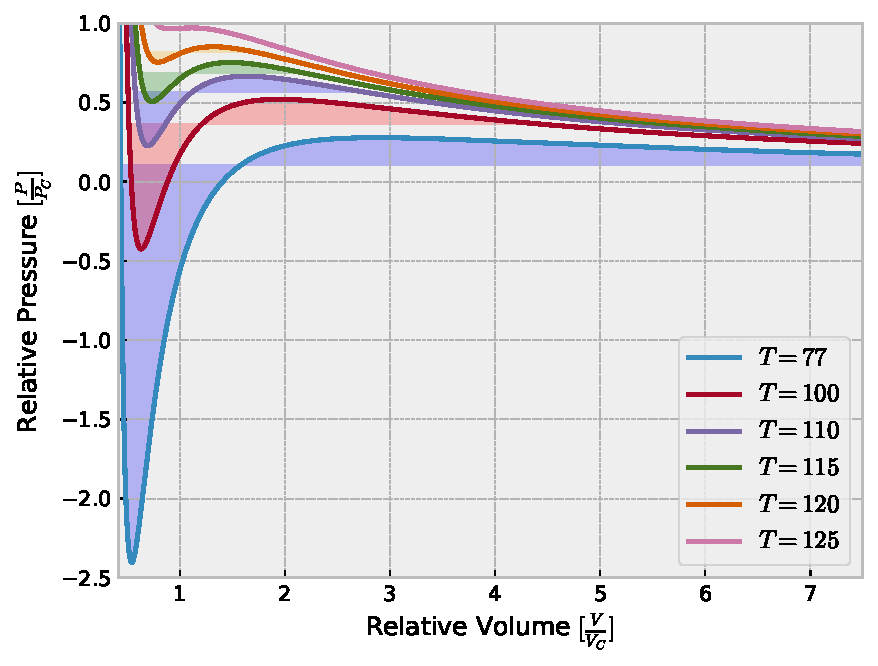
\includegraphics[width=0.8\textwidth]{../figures/equation_of_state_area.pdf}
    \caption{The Maxwell relation used for different temperatures of the wan der Waal equation of state, where the highlighted areas are the areas calculated by the trapezoidal method.}
    \label{fig:14}
\end{figure}

Using this method we can find the values for $V_g$ and $V_l$ for different temperatures. The value for $V_l$ is the volume value of where the integral starts, and $V_g$ is the value of the volume where at the first intersection between the graph and the integral. The values we found for each temperature is shown in table \vref{table_4}.\\
The code to creates this figure is shown in listing \vref{program1}.

% Please add the following required packages to your document preamble:
% \usepackage{booktabs}
\begin{table}[]
\begin{center}
\caption{Gas volume and liquid volume found by using Maxwell relation on the data showed in figure \vref{fig:14}}
\begin{tabular}{@{}lllllll@{}}
\toprule
Temperature {[}K{]} & $77$ & $100$ & $110$ & $115$ & $120$ & $125$ \\ \midrule
$V_l$ {[}$V_c${]}    & 1.58 & 1.21  & 1.12  & 1.08  & 1.04  & 0.97  \\
$V_g$ {[}$V_c${]}    & 0.44 & 0.51  & 0.57  & 0.62  & 0.69  & 0.86  \\ \bottomrule
\end{tabular}
\label{table_4}
\end{center}

\end{table}

\subsection*{1.5}
For the critical temperature the difference in liquid volume and gas volume, $V_l-V_g$, is zero. We can therefore use the data shown in table \vref{table_4} to estimate the critical temperature $T_c=127$K. By plotting the data shown in table \vref{table_4} we produce the graph shown in figure \vref{fig:15}.

\begin{figure}[h!]
  \centering
    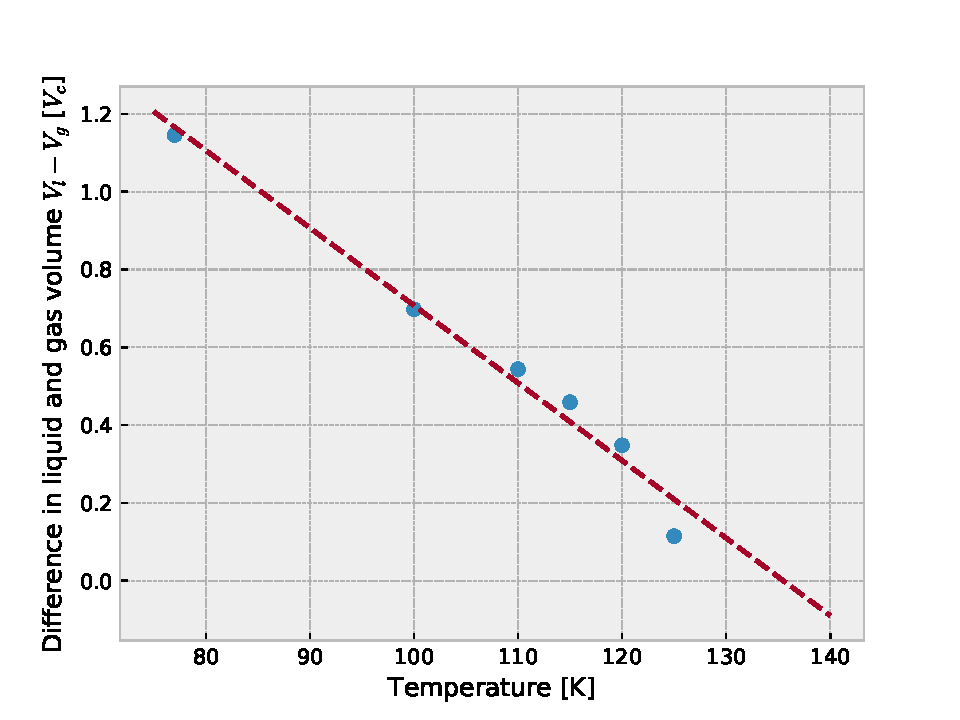
\includegraphics[width=0.8\textwidth]{../figures/lin_reg.pdf}
    \caption{The difference in gas and liquid volume as a function of temperature. The values used are the as the ones given in table \vref{table_4}. From the linear regression we can calculate for what $T$ value we have $V_g=V_l$.}
    \label{fig:15}
\end{figure}

The code to creates this figure is shown in listing \vref{program1}.
From this data we calculate the critical temperature $T_c$ by finding the intersection between the linear regression and $V_l-V_g=0$.
With this method we find the critical temperature to be $135\pm13$K, while the true value is $127$K. Where we have calculated the uncertainty from the uncertainty in the constant term and the slop of the linear regression. The true value is within the uncertainty of our result, but there is quite a large difference. This is most likely from the uncertainty in the position of $V_l$ and $V_g$, as well as the fact that van der Waal's equation is not exact.
\section*{Problem 2 - The Partition Function}
We have a particle which can only have five states, with energies
\begin{equation}
    \epsilon_i = \{-0.1, -0.05, 0, 0.05, 0.1\} \text{eV}, \label{energy_1}
\end{equation}
where $i$ is the $i$'th element in the list. The particle is in thermal equilibrium with a heat bath at room temperature, $T=300$K.
The results in this task was calculated using the program given in listing \vref{program2}.
\subsection*{2.1}
We have all the information to find the partition function $Z$ for our system
\begin{align}
    Z &= \sum_{i=1}^{5} e^{-\epsilon_i/kT} = 55.95 \label{party}
\end{align}
\subsection*{2.2}
With the partition function we can calculate the probability of measuring the particle in each energy state
\begin{equation}
    P_i = \frac{1}{Z}e^{-\epsilon_i/kT}.\label{probi}
\end{equation}
This gives us the probabilities shown in table \vref{table_1}.
\begin{table}[]
    \begin{center}
    \caption{Probabilities of different energy states with both positive and negative energies \eqref{energy_1}, calculated using the Partition function \eqref{probi}.}
    \begin{tabular}{@{}llllll@{}}
    \toprule
    State \#                & 1     & 2     & 3    & 4    & 5    \\ \midrule
    Energy {[}eV{]}      & -0.10 & -0.05 & 0    & 0.05 & 0.10 \\
    Probability {[}\%{]} & 85.55 & 12.36 & 1.79 & 0.23 & 0.04 \\ \bottomrule
    \end{tabular}
    \label{table_1}
    \end{center}
\end{table}
\subsection*{2.3}
We can, as we are allowed to do, parallel shift the energies to
\begin{equation}
    \epsilon_i = \{0, 0.05, 0.1, 0.15, 0.2\} \text{eV}, \label{energy_2}
\end{equation}
and now want to find out what quantities have changed. Using \eqref{party}
we find that the Partition function is $1.168$.
Using equation \eqref{probi} gives us the probabilities shown in table \vref{table_2}.
\begin{table}[]
    \begin{center}
    \caption{Probabilities of different energy states with only positive energies \eqref{energy_2}, parallel shifted compared to \eqref{energy_1}. The probabilities were calculated by using the Partition function \eqref{probi}.}    \begin{tabular}{@{}llllll@{}}
    \toprule
    State \#                & 1     & 2     & 3    & 4    & 5    \\ \midrule
    Energy {[}eV{]}      & 0 & 0.05 & 0.10    & 0.15 & 0.20 \\
    Probability {[}\%{]} & 85.55 & 12.36 & 1.79 & 0.23 & 0.04 \\ \bottomrule
    \end{tabular}
    \label{table_2}
    \end{center}
\end{table}
By comparing the values in table \vref{table_1}
and table \vref{table_2} we see that even though the energies are parallel shifted the probabilities are the same. The probabilities are still conserved, since the values of the partition function changed. This is the only physically acceptable outcome, since we are not changing the system by parallel shifting the energies, the probabilities should not change either. \newpage
\section*{Problem 3 - Maxwell-Boltzmann Distribution}
The Maxwell-Boltzmann distribution is given as
\begin{equation}
    D(v) = \left(\frac{m}{2\pi kT}\right)^{\frac{3}{2}}4\pi v^2e^{-\frac{mv^2}{2kT}}.
\end{equation}
All the numerical integration and plotting of figures in this problem was done by the code given in listing \vref{program3}.
\subsection*{3.1}
To find the most probable velocity we derivate the distribution with respect to velocity, and set it equal to zero.
\begin{align*}
    \pdv{D(v)}{v} &= 0 \\
    \pdv{}{v}\left(\left(\frac{m}{2\pi kT}\right)^{\frac{3}{2}}4\pi v^2e^{-\frac{mv^2}{2kT}}\right) &= 0 \\
    4\pi\left(\frac{m}{2\pi kT}\right)^{\frac{3}{2}}\pdv{}{v}\left(v^2e^{-\frac{mv^2}{2kT}}\right) &= 0 \\
    4\pi\left(\frac{m}{2\pi kT}\right)^{\frac{3}{2}} \left(2ve^{-\frac{mv^2}{2kT}}-\frac{mv^3}{kT}e^{-\frac{mv^2}{2kT}}\right) &= 0 \\
    \left(2v-\frac{mv^3}{kT}\right)e^{-\frac{mv^2}{2kT}} &= 0 \\
    2v-\frac{mv^3}{kT} &= 0 \\
    2v &= \frac{mv^3}{kT} \\
    \frac{2kT}{m} &= v^2 \\
    v &=  \sqrt{\frac{2kT}{m}}
\end{align*}
We denote the most probable velocity as $v_p$.
We now want to calculate the average velocity $\langle v \rangle $ we need to solve the following integral
\begin{equation}
    \langle v \rangle = \int_0^\infty vD(v)\diff v.
\end{equation}
Let's begin the calculation!
\begin{align*}
 \langle v \rangle &= \int_0^\infty vD(v)\diff v \\
 &= \int_0^\infty v \left(\frac{m}{2\pi kT}\right)^{\frac{3}{2}}4\pi v^2e^{-\frac{mv^2}{2kT}} \diff v \\
 &= \left(\frac{m}{2\pi kT}\right)^{\frac{3}{2}}4\pi \int_0^\infty  v^3e^{-\frac{mv^2}{2kT}} \diff v
\end{align*}
To solve this integral we search through Rottmann formula collection and find the following integral
\begin{equation}
    \int_0^\infty e^{-\lambda x^2}x^{k}\diff x = \frac{1}{2}\lambda^{-\frac{k+1}{2}}\Gamma\left(\frac{k+1}{2}\right)
\end{equation}
which we use to evaluate our integral, with the values $k=3$ and $\lambda = m/(2kT)$ we then find the following solution, where we use that $\Gamma(2) = 1$,
\begin{align*}
    \langle v \rangle &= \left(\frac{m}{2\pi kT}\right)^{\frac{3}{2}}4\pi\frac{1}{2}\left(\frac{m}{2kT}\right)^{-2}\Gamma\left(2\right) \\
    &= \sqrt{\frac{2kT}{m}}\frac{2}{\sqrt{\pi}} = \sqrt{\frac{8kT}{\pi m}} \\
    &= \frac{2}{\sqrt{\pi}}v_p
\end{align*}
We are also interested in finding the root mean square of the velocity $\sqrt{\langle v^2\rangle }$, so now we need to calculate $\langle v^2\rangle$. Let's begin!
\begin{align*}
    \langle v^2\rangle &= \int_0^\infty v^2D(v)\diff v \\
    &= \int_0^\infty \left(\frac{m}{2\pi kT}\right)^{\frac{3}{2}}4\pi v^4e^{-\frac{mv^2}{2kT}} \diff v \\
    &= \left(\frac{m}{2\pi kT}\right)^{\frac{3}{2}}4\pi \int_0^\infty v^4e^{-\frac{mv^2}{2kT}} \diff v
\end{align*}
To solve this integral we will again use Rottmann, where we find
\begin{equation}
    \int_0^\infty x^{2n} e^{-x^2/a^2} = \sqrt{\pi}\frac{\left(2n\right)!}{n!}\left(\frac{a}{2}\right)^{2n+1}
\end{equation}
where we have $n=2$, and $a=\sqrt{2kT/m}$. Let's continue
\begin{align*}
    \langle v^2\rangle &= \left(\frac{m}{2\pi kT}\right)^{\frac{3}{2}}4\pi \sqrt{\pi}\frac{4!}{2!} \sqrt{\frac{2kT}{4m}}^5 \\
    &= \left(\frac{m}{2\pi kT}\right)^{\frac{3}{2}}4\pi\sqrt{\pi}12 \sqrt{\frac{kT}{2m}}^5\sqrt{\frac{m}{2kT}}^3 \\
    &= \frac{12\cdot 4 \pi\sqrt{\pi}}{\pi\sqrt{\pi}2^{5/2}}\frac{1}{2^{3/2}}\left(\frac{kT}{m}\right)^{5/2}\left(\frac{m}{kT}\right)^{3/2} \\
    &= 3\frac{kT}{m}
\end{align*}
This means the root-mean-square value is
\begin{equation}
    v_{rms} = \sqrt{\langle v^2\rangle} = \sqrt{\frac{3kT}{m}} = \sqrt{\frac{3}{2}}v_p
\end{equation}
We have now found an expression for $\langle v \rangle$, $v_{rms}$ and $v_p$, we want to find the numerical value of this velocity for $N_2$ molecule at a temperature of $300$K and $600$K, the result is shown in table \vref{table_3}, where we used $k=8.31$J/mol K and $0.028$kg/mol.
\begin{table}[]
    \begin{center}
    \caption{Average, most probable and root-mean-square velocity for $300$K and $600$K.}
    \begin{tabular}{@{}lll@{}}
    \toprule
    Temperature {[}K{]}                               & $300$ & $600$ \\ \midrule
    $\langle v \rangle$ [m/s] & 336.7 & 476.2 \\
    $v_p$ [m/s]                                            & 298.4 & 422.0 \\
    $v_{rms}$ [m/s]                                         & 365.4 & 516.8 \\ \bottomrule
    \end{tabular}
    \label{table_3}
    \end{center}
\end{table}

\subsection*{3.2}
The distribution for the temperature $300$K and $600$K is plotted in figure \vref{fig:maxwell_dist}. Where we can see that increasing the temperature makes the value of the most probable velocity larger, as well as increasing the spread in probabilities.
\begin{figure}[h!]
  \centering
    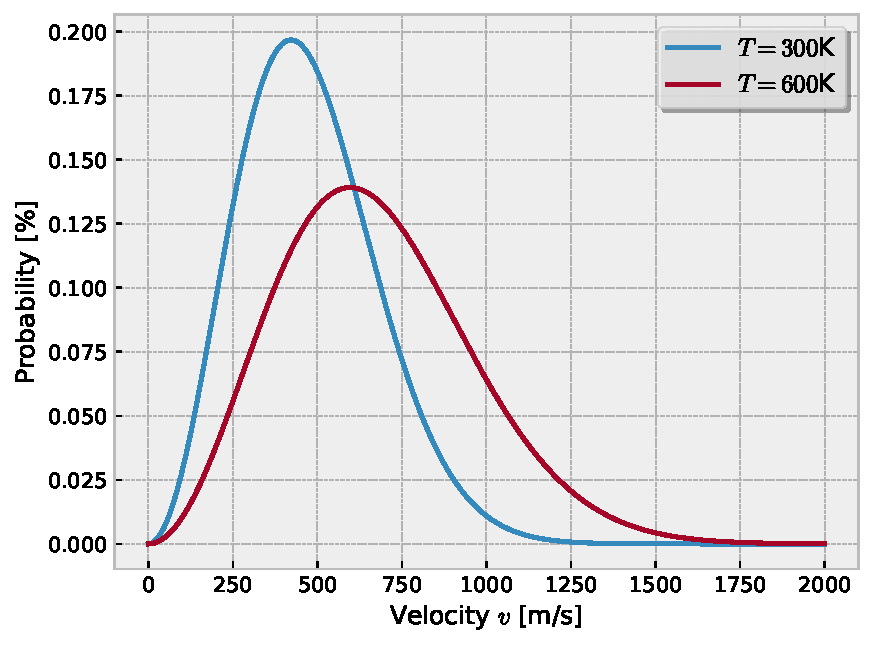
\includegraphics[width=0.8\textwidth]{../figures/MaxwellDistribution.pdf}
    \caption{Probability distribution as a function of velocity of temperatures of $300$K and $600$k}
    \label{fig:maxwell_dist}
\end{figure}

\subsection*{3.3}
We want to find the probability of of measuring an $N_2$ molecule with a speed less than $300$m/s at a temperature of $300$K. Since the integral of the Maxwell-Boltzmann distribution does not have an analytical solution with limits (except when integrating from $0$ to $\infty$), we will have to use numerical integration. We find that the probability of measuring a velocity less than $300$m/s is $20.13$\%.

\subsection*{3.4}
The temperature of Earth's atmosphere is $1000$K. The escape velocity of a particle in the atmosphere of the earth is $11 000$m/s. We want to find a probability of measuring a nitrogen particle with a velocity of more than $11000$m/s. We again calculate the integral numerically to find the probability to be $4.75\times 10^{-86}$. This probability is effectively zero, and is the reason for why the Earth has an atmosphere, since the particles are not energetic enough to escape.

\subsection*{3.5}
We now repeat the calculation, but now with Hydrogen (with a mass of $0.002$kg/mol) and Helium (with a mass of $0.004$kg/mol). We then find the respective probabilities: $2.1\times 10^{-4}$\%, $1.39\times 10^{-10}$\%. From this result we would assume that we have less hydrogen than helium in our atmosphere. On wikipedia we find that the amount of helium in our atmosphere is $0.000524\%$ and hydrogen is $0.000053\%$. This result seems reasonable when we compare to the values we found. We have also assumed that the escape velocity of a particle on earth is $11000$m/s for all heights, which is not true, and we should expect some deviation.

\subsection*{3.6}
We now do the same calculation for the moon, where the escape velocity is $2400$m/s, and again assume a temperature of $1000$K. We again calculate the probability of observing a nitrogen molecule with a velocity larger than the escape velocity to be  $0.0225$\%. This is a lot more likely compared to what we found for the Earth. We can therefore conclude that the moon should not have an atmosphere, at least not one with a temperature of $1000$K, since the particles would escape the gravitational pull.
\newpage
\section*{Code Appendix}
\subsection*{Code For Problem 1}
\lstinputlisting[label=program1,caption=Python code used to solve problem 1. And plotting the result.,language=python]{../problem1_3.py}
\subsection*{Code For Problem 2}
\lstinputlisting[label=program2,caption=Python code used to solve problem 2. And plotting the result.,language=python]{../problem2_1.py}
\subsection*{Code For Problem 3}
\lstinputlisting[label=program3,caption=Python code used to solve problem 3. And plotting the result.,language=python]{../problem3_2.py}
\end{document}
